\subsection{Implementación SRGAN.}

La implementación de este modelo se realizara utilizando la arquitectura presentada
en \cite{SRGAN} mediante el lenguaje \emph{Python} utilizando la librería de alto nivel \emph{Keras}

Keras es una API que proporciona numerosos bloques
de construcción útiles los cuales pueden ser conectados para crear arquitecturas de
aprendizaje profundo altamente complejas.

Para el entrenamiento de las redes, Keras utiliza una de las tres librerías como
\emph{backend} para este propósito: \emph{TensorFlow}, \emph{CNTK}, o \emph{Theano}. Para esta implementación
se utiliza \emph{TensorFlow}, que es una librería de Python de código abierto para el
aprendizaje automático, esta fue desarrollada por Google.

Utilizaremos el dataset MIRFLICKR \cite{MIRFLICKR} el cual es una base de datos de imágenes
extraídas de la red social flickr, esta base consta de 25000 imágenes y la principal ventaja es 
que las imágenes son muy variadas por lo cual es ideal en el entrenamiento de una red neuronal capaz 
de mejorar los detalles de una imagen. Cabe resaltar que no se utilizaron todas las imágenes del dataset
debido al tiempo de ejecución del entrenamiento, así como las limitantes de hardware al ejecutar el código.

Las imágenes originales del dataset son de una dimensión de 500x500 pixeles, para el modelo generador
se utiliza una imagen de entrada de baja resolución de 32x32 pixeles y la imagen de alta resolución de salida
será de 128x128 pixeles, teniendo un escalado de 4 veces el tamaño original. 

\subsubsection{Modelo generador.}





\begin{figure}[H]
  \begin{center}
    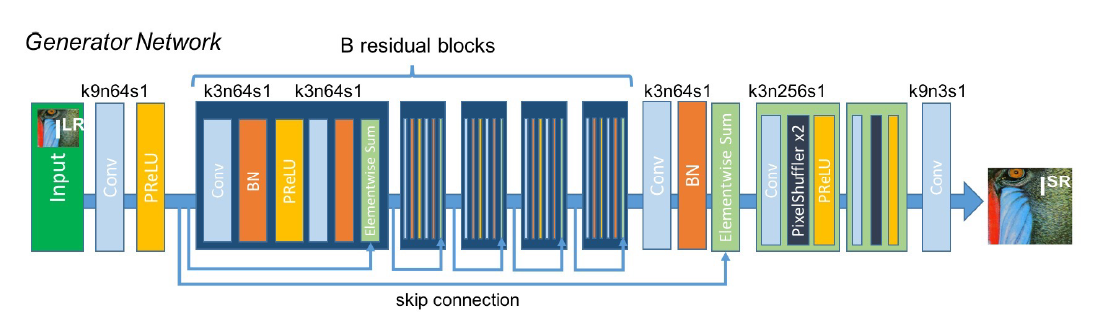
\includegraphics[scale = 0.7]{Imp_generador.png}
    \caption{Arquitectura del generador de la SRGAN,\emph{k} es el tamaño del
    filtro, \emph{n} es la dimensión del mapa de características (capa de convolución) y \emph{s} indica
    el valor del parámetro stride. Imagen tomada de \cite{SRGAN}}
    \label{Alexis4}
  \end{center}
\end{figure}

\subsubsection{Modelo discriminador.}

\begin{figure}[H]
  \begin{center}
    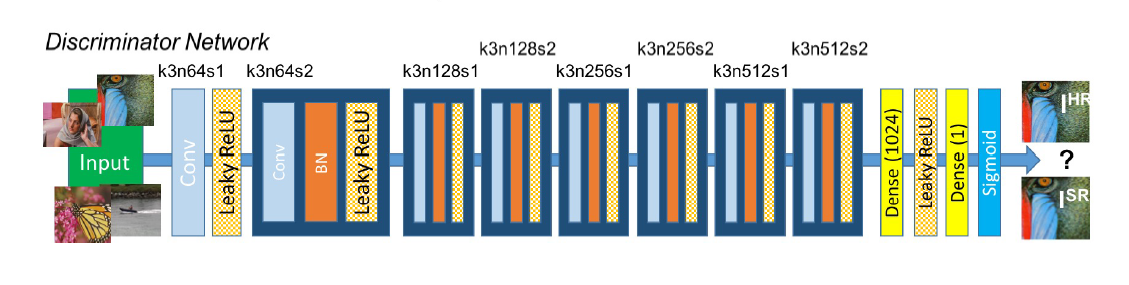
\includegraphics[scale = 0.7]{Imp_discriminador.png}
    \caption{Arquitectura del Discriminador de la SRGAN, \emph{k} es el tamaño
    del filtro, \emph{n} es la dimensión del mapa de características (capa de convolución) y \emph{s}
    indica el valor del parámetro stride. Imagen tomada de \cite{SRGAN}}
    \label{Alexis5}
  \end{center}
\end{figure}

\subsubsection{Entrenamiento}

EL modelo de entrenamiento de las GAN´s como se ha mencionado en \cite{GANs} y \cite{SRGAN}, es un proceso en el cual
los dos modelos compiten, el generador por engañar al discriminador y el discriminador por no permitirlo, en la figura \ref{Alexis6}
podemos ver el proceso en el cual se basa el entrenamiento.

\begin{figure}[H]
    \begin{center}
      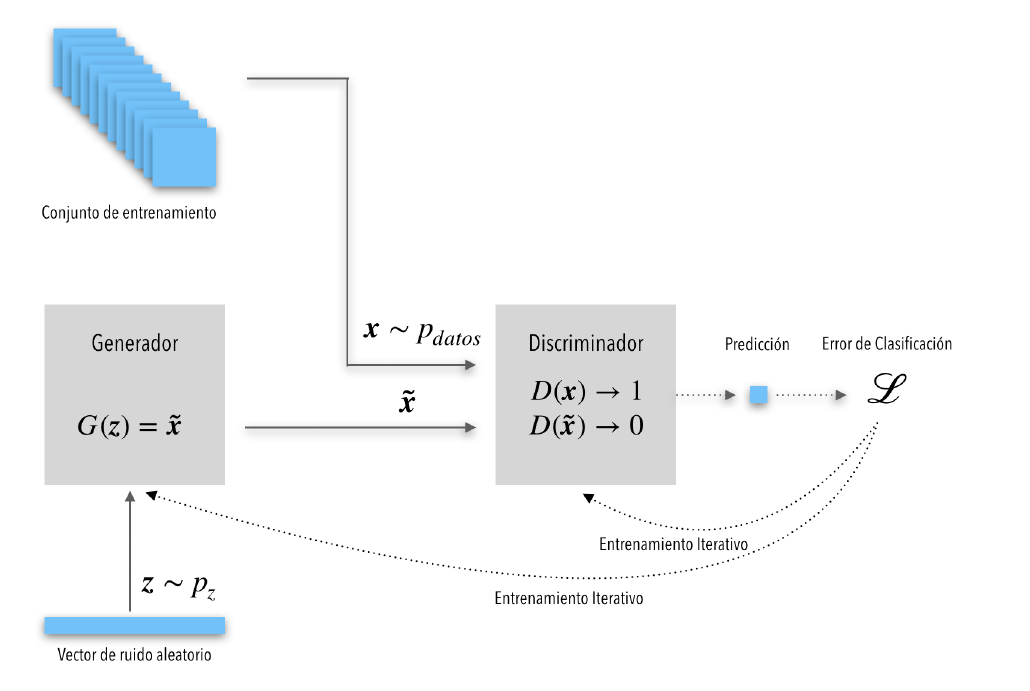
\includegraphics[scale = 0.6]{proceso_gan.png}
      \caption{Proceso de entrenamiento}
      \label{Alexis6}
    \end{center}
\end{figure}


Para lograr

\subsubsection{Métricas}
 Durante el entrenamiento se tiene

 \begin{table}[H]
  \centering
  \caption{Resultados Máximo y Mínimos de las perdidas.}
  \begin{tabular}{|l|l|l|}
  \hline
  \textbf{Criterio} & \textbf{Valor Máximo} & \textbf{Valor Mínimo}  \\ \hline
  Pérdida del Generador           & 228.5551261019351              & 23.898190839255033     \\
  Pérdida del Discriminador       & 1.236285184701566              & 1.6890162633455543e-16  \\
  Precisión Discriminador         & 1.0                            & 0.8630597014925373       \\ \hline
  \end{tabular}
\end{table}